% Chapter 2

\chapter{Présentation de l'IRMA} % 2 nd chapter title

\label{Chapter2} % For referencing the chapter elsewhere, use \ref{Chapter2} 

\textit{Les informations presentes dans cette section sont entierement issues du \href{http://irma.math.unistra.fr/}{site web de l'IRMA}}

Cree en 1966 par Jean Frenjel et Gearges Reeeb, l'IRMA\footnote{Institut de Recherche Mathématique Avancée} est une  unité mixte de recherche (UMR 7501) sous la double tutelle du CNRS (a travers l'INSMI\footnote{Institut National des Sciences Mathématiques et de leurs Interactions}) et de l’Université de Strasbourg (UFR de Mathématique et d’Informatique).

Dirigee par le professeur Philippe Helluy, l'IRMA comporte environ 130 membres. On y compte enviro 87 chercheurs et enseignants-chercheurs permanent et une qurantaine de non permanents repartis en 8 equipes de recherche.

Les activites majeures de l'organisme sont l'organisation des seminaires, des journees, des colloques et des conferences. Ces activites sont renforcees par les nombreux partenariats qu'elle maintient dans les secteurs academique(Cemosis, Labex IRMIA, etc..) et indutriel (AxesSIM, Electis, etc..).

%----------------------------------------------------------------------------------------

\section{Structure de l'organisation}
L'organigramme de l'entreprise representant ses sections majeures est donne a la figure \ref{fig:OrganigrammeIRMA}).

\begin{figure}[!h]
\centering
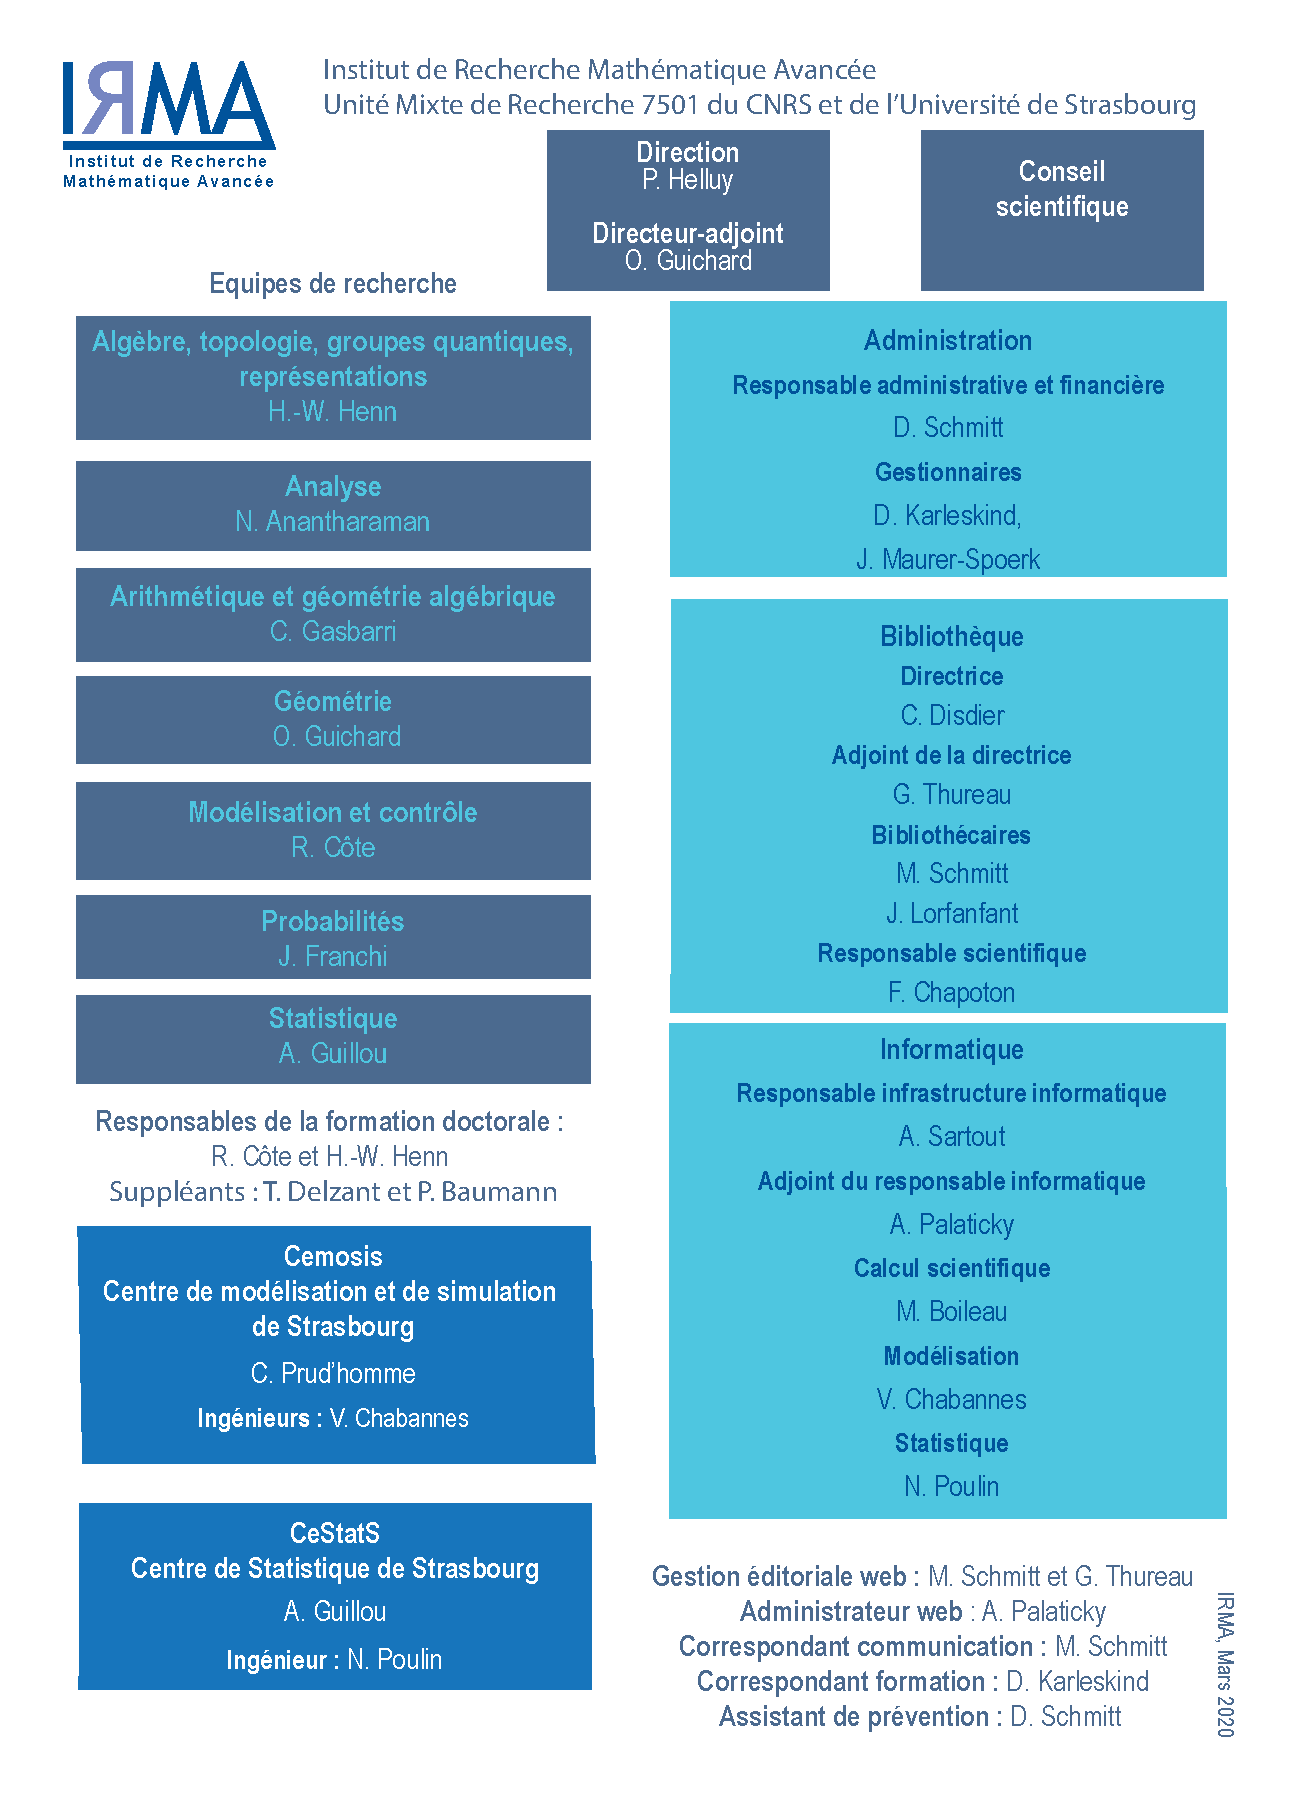
\includegraphics[width=.8\linewidth]{OrganigrammeIRMA} 
\decoRule
\caption[Organigramme de l'IRMA]{Organigramme representant l'organisaiton de l'IRMA au mois de mars 2020 \parencite{Reference7}}
\label{fig:OrganigrammeIRMA}
\end{figure}

%----------------------------------------------------------------------------------------

\section{Les équipes MOCO et Probabilite}

L'equipe MOCO \footnote{MOdelisation et COntrole} se compose de specilistes des EDP, de la theorie deu controle, ddu calcul scientifique et haute performance et des statistiques. Ses activites s'etendent a l'internationale et dans l'indutriel (REF, ...). Les enseignants-chercehurs MM. Emmanuel Franck et en Laurent Navoret y sont responsables des seminaires en equations aux derivees partielles. 

L'equipe probabilite est composee d'experts en calcul de probabilite. Ses membres se retrouvent regulierement lors du "seminaire stochatique". A cette equipe apartient M. Vincent Vigon. 

Je tiens une fois de plus a remercier les trois chercheurs mentiones ci-hauts qui ont encadrer ce stage. La combinaison de ces deux equipes dont ils font partie a permis de faire face aux deux aspects de ce stage. Premierement la modelisation d'EDP et finalement l'utilisation des reseaux de neurones.

%----------------------------------------------------------------------------------------
